\section{Considerações Iniciais}


Neste contexto, uma premissa fundamental é manter todas as visões/artefatos do metamodelo KDM sincronizados durante todo o processo de modernização do software. Dessa forma, quando as visões/artefatos representados em nível de modelos são alterados, é de extrema importância realizar um conjunto de propagação de mudança por todas as visões/artefatos para mantê-los atualizados e sincronizados, espelhando assim, a alteração em todas as visões/artefatos do software. Usualmente, como apresentado nos Capítulo~\ref{chapter:fundamentacao_teorica}, Seção~\ref{sec:refatoracao} e Capítulo~\ref{chapter:catalogo_refactoring_KDM} essas alterações podem ser realizadas por meio de refatorações, as quais são atividades centrais durante o processo de modernização. Porém, quando um software é representado utilizando diferentes abstrações e visões em nível de modelos, um acidente comum que pode ocorrer durante a atividade de refatoração é a dessincronização dessas visões, fazendo com que as visões/artefatos que representam o sistema fiquem inconsistente após a atividade de refatoração. Uma forma de resolver esse problema é aplicar técnicas de propagação de mudança, cujo objetivo é identificar e atualizar todas as instâncias dependentes dos elementos que foram refatorados. % No entanto, a maioria das propostas de propagação de mudança foram desenvolvidas para propagarem mudanças em diferentes metamodelos, além disso, usualmente tais metamodelos são de diferentes fornecedores dificultando o entendimento e a programação de mudança (ref). 
Diante deste contexto, neste capítulo é apresentado uma abordagem para realizar a propagação de mudança e preservação de comportamento após a aplicação de refatorações em instâncias do metamodelo KDM. Utilizando a abordagem aqui definida, modernizadores podem se concentrar apenas no desenvolvimento das refatorações ou reutiliza-las por meio do metamodelo SRM (ver Capítulo~\ref{chapter:Toward_a_Refactoring_Metamodel_for_KDM}), sem terem que se preocuparem com a propagação de mudanças para outras visões/artefatos do metamodelo KDM. 

É importante destacar que o fluxo da abordagem inicia-se considerando que o engenheiro de software almeja aplicar um conjunto de refatorações em um sistema que está já representado por meio de uma instância do metamodelo KDM. Essa instância do metamodelo KDM deve ser a mais completa possível, ou seja, represente todas as visões/artefatos do sistema, desde o código-fonte até os elementos arquiteturais do sistema\footnote{Na verdade é importante que mais de uma visão/artefato seja representado utilizando o metamodelo KDM, seja código-fonte, banco de dados, elementos estruturais, etc.}. Após o engenheiro de software aplicar uma determinada refatoração, a abordagem, a qual contém três principais passos, efetivamente é iniciada. De forma resumida pode-se descrever os três passos da abordagem da seguinte forma. 

O primeiro passo da abordagem realiza uma comparação (do inglês - \textit{diff}) entre a instância refatorada do metamodelo KDM com a instância do metamodelo KDM original, ou seja, a instância do metamodelo KDM antes do modernizador aplicar a refatoração. Como resultado, esse passo cria uma lista que contém todas as instâncias das metaclasses do KDM que sofreram uma modificação durante a refatoração quando comparado com a instância do KDM original. Em seguida, o segundo passo utiliza como entrada a lista gerada para ser utilizada como parâmetro para um algoritmo de mineração e identificação de dependências. Esse algoritmo tem como objetivo identificar todas as instâncias das metaclasses do KDM que possuem dependência com as metaclasses refatoradas. Como resultado, esse algoritmo também cria uma lista, a qual é utilizada no terceiro passo. O terceiro passo utiliza a lista criada pelo algoritmo para realizar um conjunto de transformações em nível de modelo. Tais transformações foram pré-definidas e representam a propagação de mudança por todas as visões do KDM. É importante destacar que a abordagem foi definida com a preocupação de ser uma forma genérica e desacoplada. Assim, a abordagem pode ser aplicada em um grande conjunto de refatorações fazendo com que o modernizador não tenha que se preocupar com a propagação de mudança para outras visões/artefatos do KDM. 

As demais seções deste capítulo estão organizadas da seguinte forma: na Seção~\ref{sec:kdm_sinc} a abordagem KDM-SInc é descrita, na Subseção~\ref{sec:diff_entre_kdm} o primeiro passo da abordagem KDM-SInc é apresentado, o segundo passo é apresentado na SubSeção~\ref{subsec:identificandoPontoParaExecutarApropagacao}, e na Subseção~\ref{subsec:aplicar_propagacao_KDM-SInc}. Na Seção~\ref{sec:consideracoes_finals_kdm_sinc} as considerações finais deste capítulo são apresentadas.


\section{A Abordagem KDM-SInc}\label{sec:kdm_sinc}

Um problema critico durante a modernização de software diz respeito a propagação de mudança - por exemplo,  dado um conjunto de refatorações que são aplicadas durante a modernização de software é importante identificar quais são as mudanças que precisam ser realizadas para manter a consistência e sincronia de todos os artefatos do sistema. Dessa forma, propagação de mudança é uma técnica de extrema importância durante a elaboração de processo de modernização de software. O engenheiro de modernização tem que ter a certeza que a refatoração foi corretamente propagada e que o software não possui nenhuma inconsistência. Embora muitas abordagens de propagações de mudanças possam ser identificadas na literatura, a propagação de mudanças ainda é um desafio durante a manutenção e modernização de software~\cite{Tom_2008_roadmap}. Além disso, a maioria das abordagens de propagação de mudanças existentes têm como principal artefato o código-fonte~\cite{Vaclav_methodology, Deursen07model_drivensoftware}. Similarmente também é possível identificar algumas abordagens que dão suporte para a propagação de mudança para a UML~\cite{Egyed_2008,Liu02rule, Briand_2006}. Porém, até o momento nenhuma abordagem ou iniciativa foi criada para o metamodelo KDM. Para suprir essa limitação nessa seção a abordagem denominada KDM-SInc é apresentada. Essa abordagem tem como objetivo propagar mudanças por todas as visões/artefatos do metamodelo KDM para mantê-lo atualizado e sincronizado após a aplicação de uma refatoração. A intenção é criar uma abordagem que mantenha uma determinada instância do metamodelo KDM consistente e sincronizada entre todas as visões/artefatos do metamodelo KDM após a aplicação de uma determinada refatoração. 

Na Figura~\ref{fig:kdm_sinc} é apresentado uma visão geral da abordagem KDM-SInc. Como pode ser observado a abordagem KDM-SInc contempla três principais passos, os quais estão contidos em um módulo de propagação (caixa cinza). Antes de iniciar o módulo de propagação uma atividade de refatoração deve ser realizada como apresentado na Figura~\ref{fig:kdm_sinc} lado esquerdo caixa branca. A atividade de refatoração esta fora do escopo da abordagem KDM-SInc, assim, é de responsabilidade do engenheiro de modernização criar e/ou reutilizar refatoração para o metamodelo KDM e aplica-la em uma instância do metamodelo KDM. A única restrição da abordagem KDM-SInc é que duas versões da instância do metamodelo KDM seja utilizada como entrada para a abordagem - uma versão que representa a instância do metamodelo KDM antes da aplicação das refatorações (\aspas{instância original}) e outra versão que representa uma instância do metamodelo KDM após a aplicação de \textit{n} refatorações (\aspas{instância refatorada}). No contexto deste capítulo é importante entender que uma \aspas{instância original} do metamodelo KDM, é aquela que ainda não foi refatorada, também é denominada de \aspas{KDM esquerdo}, similarmente, a \aspas{instância refatorado} do metamodelo KDM pode ser entendida como \aspas{KDM direito}. 

\begin{figure}[h]
	\centering
	% Requires \usepackage{graphicx}
	\caption{Visão Geral da Abordagem KDM-SInc.}
	\label{fig:kdm_sinc}
	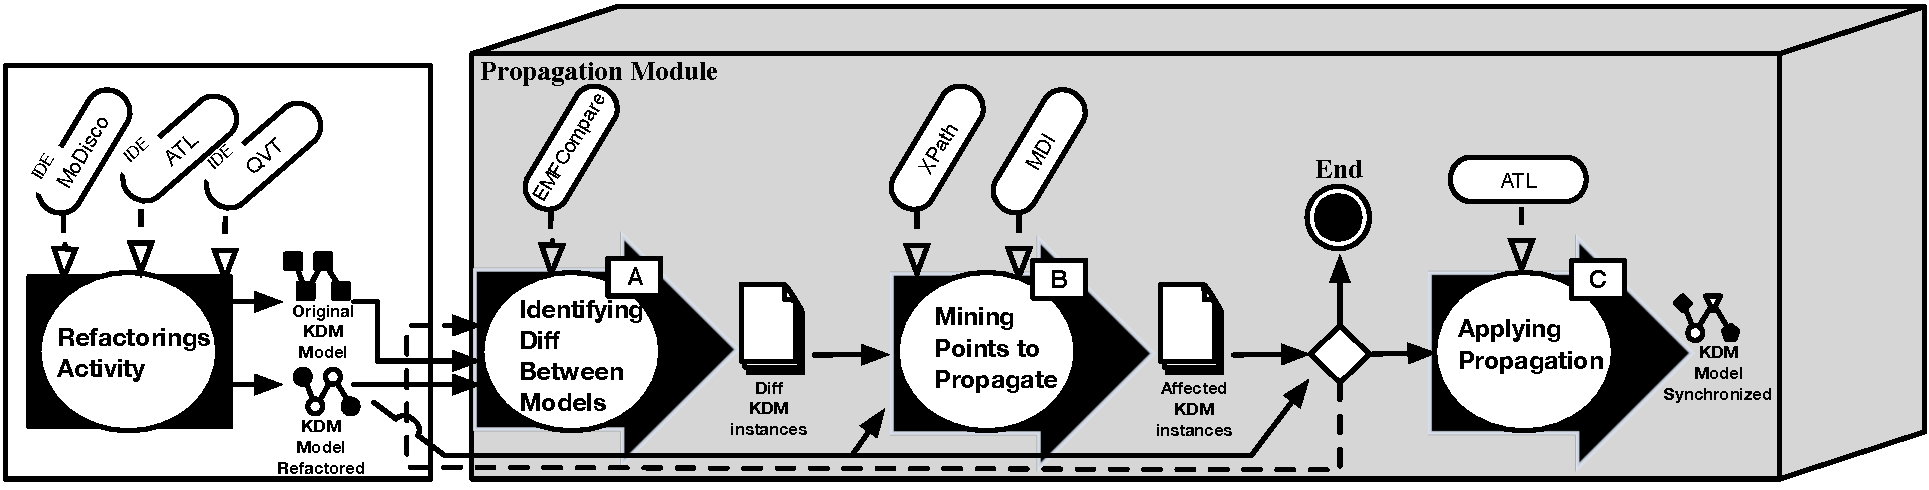
\includegraphics[scale=0.5]{images/ApproachLifeCicle2}
	\fautor
\end{figure}

Após a aplicação de um conjunto de refatorações o passo [A] pode ser iniciado. Nesse passo uma comparação (\textit{diff}) entre a instância original e a instância refatorada é realizada. Como resultado desse passo uma lista é crida. Essa lista contém todas as instâncias das metaclasses do KDM que sofreram alguma modificação durante a refatoração quando comparado com a instância do KDM original. Além disso, essa lista também especifica qual(is) foi(ram) a(s) modificação(ões) realizada(s). Por exemplo, se na versão refatorada (\aspas{KDM direito}) uma nova instância da metaclasse \texttt{ClassUnit} foi adicionada a lista irá conter duas importantes informações: (\textit{i}) a instância da metaclasse \texttt{ClassUnit} e (\textit{ii}) qual operação foi realizada, nesse exemplo \texttt{add} \texttt{ClassUnit}. Essas duas informações são importantes para identificar o que foi alterado e qual operação foi realizada (neste caso uma \texttt{ClassUnit} foi adicionada) - assim, é possível identificar quais propagações devem ser realizadas nas outras visões/pacotes do metamodelo KDM.

Em seguida o passo [B] é iniciado, o qual identifica todas as metaclasses que precisam ser sincronizadas/atualizadas após a aplicação da refatoração. Nesse passo utiliza o algoritmo de busca em profundidade (do inglês - \sigla{DFS}{\textit{Depth-First Search}}). Para a abordagem KDM-SInc o algoritmo DFS foi alterado para utilizar como entrada a lista criada no passo [A] e também a instância refatorado do KDM (\aspas{KDM direito}). Utilizando a instância refatorado o algoritmo DFS identifica e cria uma lista contendo todas as metaclasses que possuem dependência com as metaclasses que efetivamente foram refatoradas.

Posteriormente o passo [C] pode ser iniciado para realizar a propagação das mudanças na instância do metamodelo KDM. Como entrada esse passo utiliza todas as metaclasses que possuem dependência com as metaclasses que foram refatoradas (lista criada no passo [B]). As propagações de mudanças são um conjunto de regras pré-definidas que são realizadas de acordo com a instância alterada (\texttt{Package}, \texttt{ClassUnit}, \texttt{MethodUnit}, \texttt{StorableUnit}, etc) e sua operação atômica (\texttt{add}, \texttt{delete} e \texttt{change}). Após o término do passo [C] todas as visões/artefatos da instância do metamodelo KDM estão sincronizadas e consistentes.

É importante salientar que os três passos da abordagem KDM-SInc são executados várias vezes até que não haja mais elementos que precisem ser atualizados/sincronizados. Esse ciclo é necessário uma vez que uma determinada instância do metamodelo KDM pode ainda exigir propagações em outros artefatos/visões, por isso, cada ciclo da abordagem KDM-SInc se concentra apenas no próximo nível de propagação. A condição de parada da abordagem KDM-SInc é quando o algoritmo, definido no passo [B], retornar uma lista vazia, indicando que não há mais elementos que precisam ser modificados.

Para auxiliar a elaboração do passo [A] o \textit{framework} EMFCompare\footnote{https://www.eclipse.org/emf/compare/} foi estendido para comparar instâncias do metamodelo KDM. O passo [B] é tecnicamente apoiado por um motor de busca cuja parte central é o algoritmo DFS juntamente com um conjunto de expressões definidas em XPath que são executadas em uma instância do metamodelo KDM para obter todos os pacotes do KDM. Finalmente, o passo [C] é apoiado por um motor de propagação, o qual utiliza um conjunto de transformações pré-definidas em ATL para executar as propagações. Todas as propagações foram definidas com base nas operações atômicas (\texttt{add}, \texttt{delete} e \texttt{change}) apresentadas no Capítulo X \change{Mudar aqui}. Dessa forma, quando um conjunto de refatorações são executadas um conjunto de propagações bem definidas podem ser executadas no contexto de instâncias do metamodelo KDM. Maiores detalhes sobre da passo da abordagem KDM-SInc são apresentados nas próximas seções.

\subsection{Identificando \textit{Diff} entre Instâncias do Metamodelo KDM}\label{sec:diff_entre_kdm}

Nessa seção o primeiro passo da abordagem KDM-SInc é apresentado. Como já salientado o primeiro passo da abordagem KDM-SInc utiliza o \textit{framework} EMFCompare. Esse \textit{framework} foi escolhido pois o mesmo pode ser facilmente adaptado e estendido. Especificadamente o passo [A] da abordagem KDM-SInc realizada três sub-passos: (\textit{i}) \textit{Matching}, (\textit{ii}) \textit{Diffing} e (\textit{iii}) Análise dos \textit{Diffs} como apresentado na Figura~\ref{fig:diff_emf_compare}. 

Com pode ser observado na Figura~\ref{fig:diff_emf_compare} o primeiro sub-passo, \textit{matching}, necessita de duas instâncias do metamodelo KDM - uma instância original (\aspas{KDM esquerdo}) denominada \textbf{versão 1} na Figura~\ref{fig:diff_emf_compare} e uma instância refatorada (\aspas{KDM direito}) \textbf{versão 2} na Figura~\ref{fig:diff_emf_compare}. Dado as duas instâncias do metamodelo KDM, os correspondentes elementos nas duas versões do metamodelo KDM são identificados. Os correspondentes elementos são identificados por meio de identificadores únicos tais como XMI IDs. Por exemplo, na Figura~\ref{fig:diff_emf_compare} pode-se observar que a instância da metaclasse \texttt{ClassUnit} Artista apresentada na \textbf{versão 1} corresponde a instância da metaclasse \texttt{ClassUnit} Artista na \textbf{versão 2}. Para as instâncias das metaclasses \texttt{ClassUnit} Ator e \texttt{Extends} na \textbf{versão 2}, no entanto, nenhum elemento correspondente foi identificado na \textbf{versão 1}. Note que para cada elemento correspondente identificado, ou não identificado, um elemento \textit{match} é criado que será utilizado no sub-passo seguinte.

\begin{figure}[h]
	\centering
	% Requires \usepackage{graphicx}
	\caption{Visão Geral da Execução do Primeiro Passo da Abordagem KDM-SInc.}
	\label{fig:diff_emf_compare}
	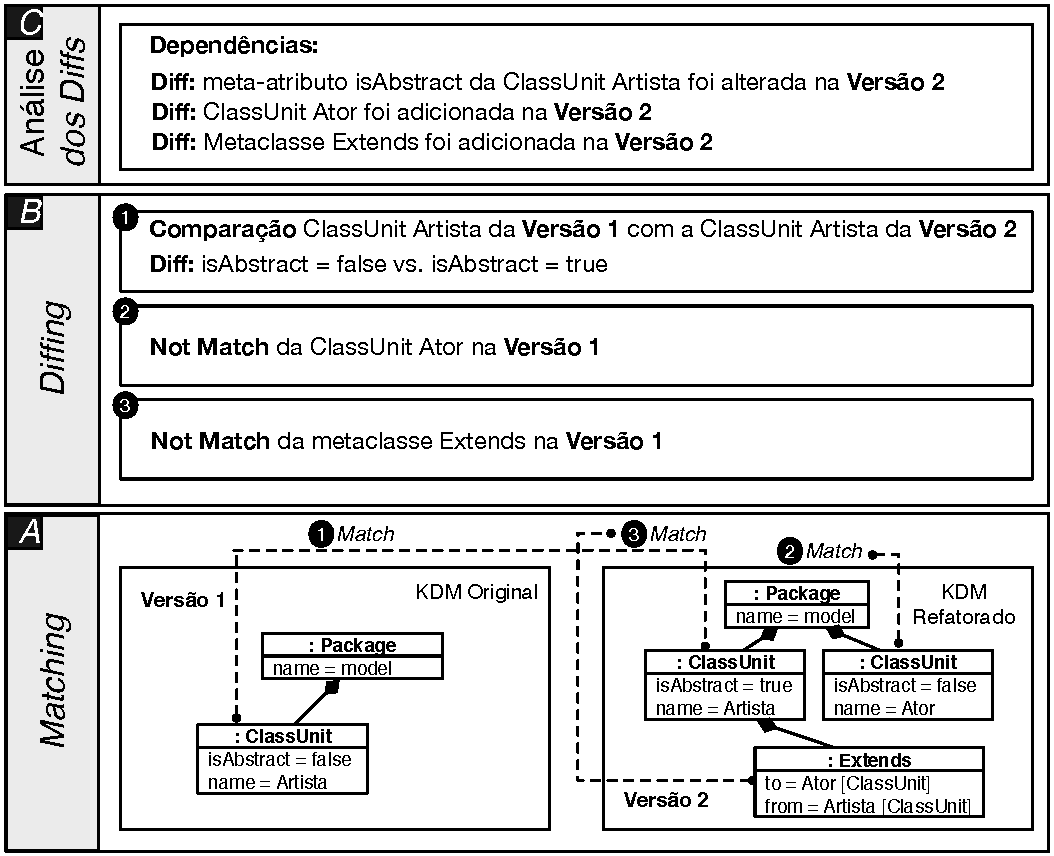
\includegraphics[scale=0.8]{images/matching_diffing_analise_3}
	\fautor
\end{figure}

No segundo sub-passo, \textit{Diffing}, todos os correspondentes elementos identificados são examinados para identificar diferenças em seus meta-atributos. Para cada diferença identificada um objeto \textit{diff} é criado, o qual descreve com precisão cada diferença entre os correspondentes elementos. Por exemplo, ainda considerando a Figura~\ref{fig:diff_emf_compare}, quando a instância da metaclasse \texttt{ClassUnit} Artista da \textbf{versão 1} e \textbf{versão 2} são examinadas é possível observar que o meta-atributo \texttt{isAbstract} possui o valor \textit{false} na \textbf{versão 1}, enquanto que na \textbf{versão 2} o mesmo meta-atributo o valor é \textit{true} - representa a operação \texttt{change}. Instâncias de metaclasses que não contêm elementos correspondentes em ambas as versões são consideradas adicionadas ou deletadas (\texttt{add} e \texttt{delete}) - a operação é identificada dependendo da direção, por exemplo, se uma instância de uma metaclasse apenas existe do lado direito (\aspas{KDM direito}) essa instância foi adicionada, por outro lado, se uma instância apenas existe do lado esquerdo (KDM esquerdo) essa instância foi deletada. Na Figura~\ref{fig:diff_emf_compare} é possível identificar que duas instâncias foram adicionadas - uma instância da metaclasse \texttt{ClassUnit} denominada Ator e uma instancia da metaclasse \texttt{Extends}.

Em seguida o terceiro sub-passo, Análise dos \textit{Diffs} é executado. Nesse sub-passo todos os objetos \textit{diffs} criados anteriormente são examinados para criar uma lista de dependência contendo as instâncias das metaclasses alteradas e quais operações foram realizadas. No exemplo apresentado na Figura~\ref{fig:diff_emf_compare} a lista criada possui três dependências. A primeiro dependência informa que o meta-atributo \texttt{isAbstract} da metaclasse \texttt{ClassUnit} Artista da \textbf{versão 1} foi alterado (\texttt{change}) de \textit{false} para \textit{true} na \textbf{versão 2}. A segunda dependência ilustra que uma instância da metaclasse \texttt{ClassUnit} Ator foi adicionada (\texttt{add}) na \textbf{versão 2} e a terceira dependência representa que uma instância da metaclasse \texttt{Extends} foi adicionada na \textbf{versão 2}.


\subsection{Identificando Pontos para Executar a Propagação}\label{subsec:identificandoPontoParaExecutarApropagacao}

Nessa seção o segundo passo da abordagem KDM-SInc é apresentado. Esse passo resume-se basicamente na adaptação do algoritmo DFS para identificar todas as metaclasses que precisam ser sincronizadas/atualizadas após a aplicação da refatoração. Esse algoritmo utiliza como entrada a lista criada no passo anterior. Como as instâncias do metamodelo KDM são persistidas utilizando a padronização XMI o algoritmo precisar de uma forma para buscar as dependências nesse XMI. Assim, esse passo utiliza expressões em XPath que são executadas na instância do metamodelo KDM para obter todos os pacotes do KDM. Por exemplo, na Figura~\ref{fig:xpath_queries} é apresentado algumas expressões definidas em XPath que é utilizada antes da aplicação do algoritmo DFS. A primeira expressão retorna a metaclasse \texttt{Segment} que é o elemento inicial de qualquer instância do metamodelo KDM. As outras expressões ilustradas nas linhas 2-5 representam os outros pacotes do metamodelo KDM. Os elementos retornados nas expressões XPath são também utilizadas como entrada para o algoritmo DFS.

\begin{figure}[h]
	\centering
	% Requires \usepackage{graphicx}
	\caption{Expressões definidas em XPath para obter os pacotes do KDM.}
	\label{fig:xpath_queries}
	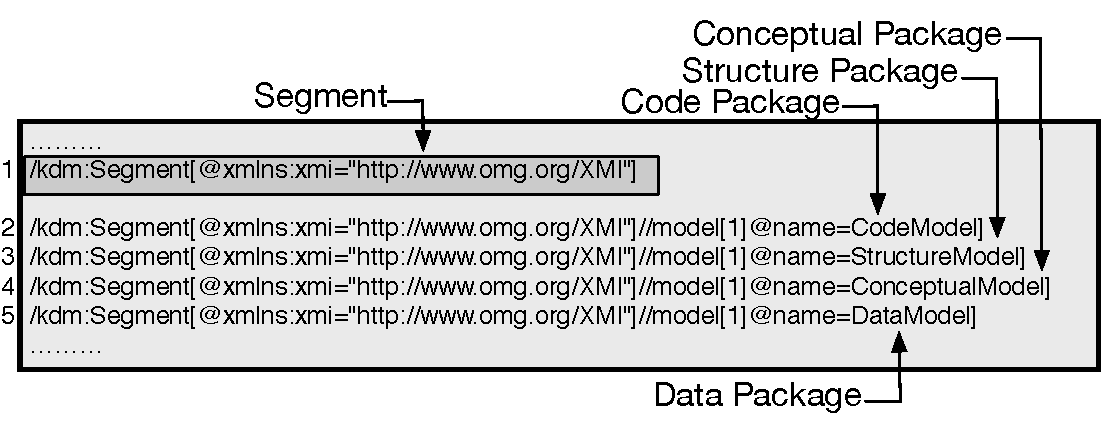
\includegraphics[scale=0.68]{images/queiresANDATLSBESNew}
	\fautor
\end{figure}

Algoritmo~\ref{alg:death1} ilustra como o DFS identifica todas as metaclasses que precisam ser sincronizadas/atualizadas após a aplicação da refatoração. A Figura~\ref{fig:dfsalg} apresenta como é o funcionamento do algoritmo DFS. Cada nó representa uma instância de uma metaclasse do metamodelo KDM os vértices representam os relacionamentos entre as instâncias das metaclasses, por exemplo, o nó \texttt{A} representa uma instância da metaclasse \texttt{Segment} e os nós \texttt{K}, \texttt{H}, \texttt{E} e \texttt{B} representam instâncias das metaclasses \texttt{CodeModel}, \texttt{StructureModel}, \texttt{ConceptualModel} e \texttt{DataModel}, respectivamente. Mais especificadamente o algoritmo funcionada da seguinte forma: primeiro é necessário escolher um ponto inicial de partida, no caso da nossa abordagem o ponto inicial é a metaclasse \texttt{Segment}, metaclasse raiz de qualquer instância do metamodelo KDM. Em seguida a metaclasse \texttt{Segment} deve ser visitada, adicionada em uma pilha e marcada como visitada. Posteriormente, o algoritmo visita uma outra metaclasse que ainda não foi visitada e verifica se a mesma possui uma associação do tipo \texttt{implementation}. Caso afirmativo, o algoritmo deve verificar se essa associação possui referência para algum elemento identificado na lista gerada no passo [A], caso a associação contenha um elemento o mesmo deve ser adicionado em um outra pilha e marcado como visitado. Todo esse processo continua até que o algoritmo alcance a ultima metaclasse. 



\begin{algoritmo}[h]
     \SetAlgoLined
     \KwIn{DFS (G, u) onde \textit{G} é uma instância do  KDM, \textit{u} é a metaclasse inicial obtida pela expressão XPath, ou seja, \texttt{Segment}}
     \KwOut{Uma coleção de metaclasses que precisam ser sincronizadas}
     \Begin{
     \ForEach{$outgoing$ edge e = (u, v) of u} {
	\If{vertex v as has not been visited}{
			\If{vertex v contain implementation = true }{
				
				\ForEach{$implementations$ element}{
				verify all elements in implementation
				}
				Mark vertex v as visited (via edge e).
				Recursively call DFS (G, v).
			}
			
				}				
			}		
	
	}
     \caption{Algoritmo DFS.}
     \label{alg:death1}
   \end{algoritmo}

Em seguida o algoritmo ainda verifica se a instância da metaclasse \texttt{Segment} possui alguma instância adjacente que ainda não foi marcada como visitado. Caso o algoritmo identifique uma instância de metaclasse adjacente ainda não visitada todo o processo é iniciado novamente, sempre verificando a associação \texttt{implementation}. Quando o algoritmo finalmente alcança a ultima instância da metaclasse, ou seja, todas as instâncias de metaclasse do KDM foram visitadas e verificadas corretamente, o algoritmo cria uma lista contendo todas as instâncias das metaclasses afetadas na refatoração. 
   
\begin{figure}[h]
	\centering
	% Requires \usepackage{graphicx}
	\caption{Funcionamento do Algoritmo DFS.}
	\label{fig:dfsalg}
	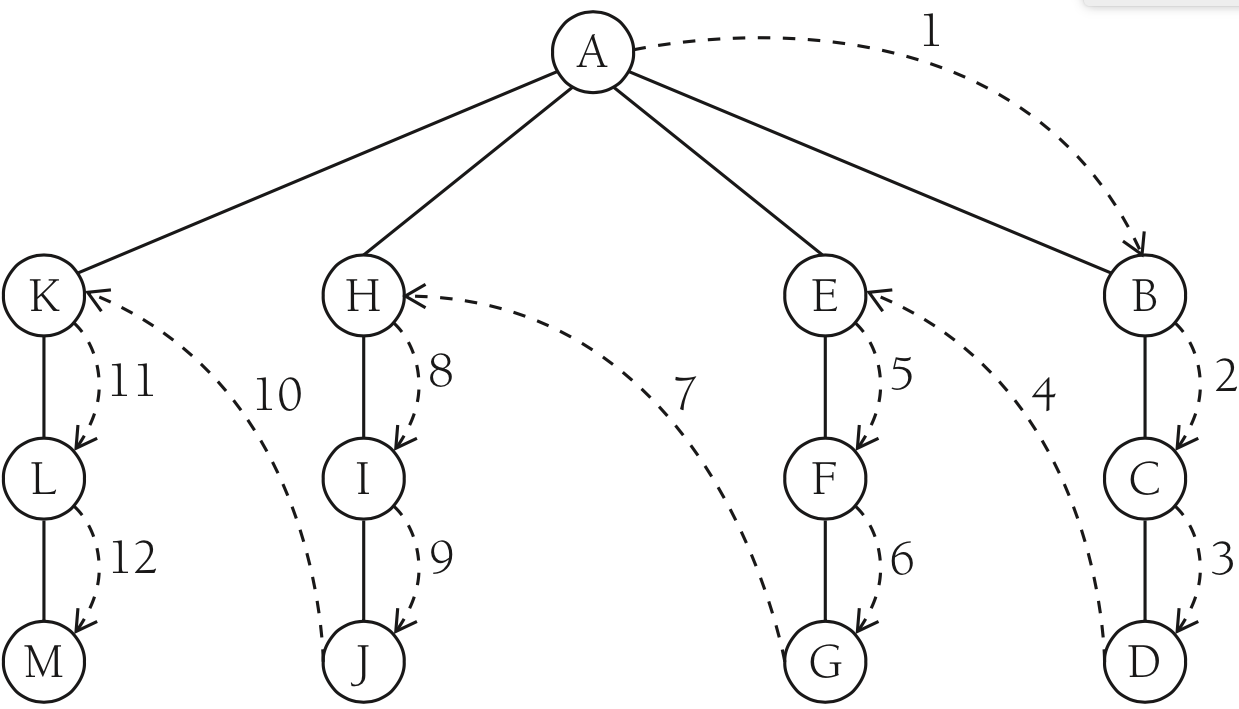
\includegraphics[scale=0.3]{images/algWorks2}
	\fautor
\end{figure}

\subsection{Aplicando Propagação}\label{subsec:aplicar_propagacao_KDM-SInc}
Nesta seção o terceiro passo da abordagem KDM-SInc é apresentado. Esse passo objetiva realizar as mudanças e propagações necessários para manter uma determinada instância do metamodelo KDM sincronizada e consistente. A sincronização é importante para o metamodelo KDM uma vez que o mesmo possui metaclasses que contêm conexões diretas com outras metaclasses de outras visões/artefatos do KDM. Assim, manter a instância do metamodelo KDM sincronizado e consistente após a aplicação de uma refatoração é importante. 

No contexto desta Tese, como apresentado no Capítulo~\ref{chapter:catalogo_refactoring_KDM} as refatorações que são definidas e adaptadas para o metamodelo KDM são refatorações de baixa granularidade e que são aplicadas diretamente na camada \texttt{Code} do metamodelo KDM. Porém, uma determinada refatoração pode demandar outras modificações que deveriam ser realizadas em outros camadas/visões do metamodelo KDM para mantê-lo consistente e sincronizado. Por exemplo, considere a refatoração \textit{Rename Package} - o nome de um determinado pacote é alterado de PacoteX para PacoteY, se uma instância da metaclasse \texttt{Layer}\footnote{Metaclasse definida no pacote \texttt{Structure} do metamodelo KDM para representar camadas em nível arquitetural.} é utilizada para representar o pacote em nível arquitetural, então essa mesma instância da metaclasse \texttt{Layer} também deve-se ser renomeada. 

Diferentemente da atividade de refatoração apresentada no Capítulo~\ref{chapter:catalogo_refactoring_KDM} onde o engenheiro de modernização precisa escolher qual refatoração aplicar na instância do metamodelo KDM ou reutilizar um refatoração utilizando o metamodelo SRM apresentado no Capítulo~\ref{chapter:Toward_a_Refactoring_Metamodel_for_KDM}, esse passo utiliza um conjunto de regras pré-definidas que são iniciadas de acordo a(s) refatoração(ões) aplicada(s) na instância do metamodelo KDM. Mais especificadamente, todas as propagações especificadas nesse passo são pré-definidas para serem disparadas após a aplicação de específicas refatorações. Algumas propagações são realizadas sem a interferência do engenheiro de modernização, no entanto, existem propagações que precisam de informações importantes para realizar consistentemente a propagação. Assim, algumas propagações podem ser realizadas de forma totalmente automática, enquanto outras precisam de algumas informações antes de executar a propagação propriamente dita.

Esse passo da abordagem KDM-SInc utiliza um conjunto de regras pré-definidas para propagar todas as mudanças em uma instância do metamodelo KDM com o intuito de mantê-lo consistente e sincronizado com todas as visões/artefatos. Todas as propagações são definidas com base nas mudanças realizadas em um determinada instância de metaclasses do metamodelo KDM. Todas as regras foram implementadas em ATL. Nas Tabelas~\ref{tab:propagacaoes_kdm_sinc_package},~\ref{tab:propagacaoes_kdm_sinc_classUnit},~\ref{tab:propagacaoes_kdm_sinc_StorableUnit} e \ref{tab:propagacaoes_kdm_sinc_method} todas as regras de programação pré-definidas são ilustradas.  

Na Tabela~\ref{tab:propagacaoes_kdm_sinc_package} as regras que representam as propagações pré-definidas para refatorações realizadas em instâncias da metaclasse \texttt{Package} são apresentadas.

\begin{longtable}{ | m{1.9cm} | m{3.57cm}| m{9.3cm} | }
 \caption{Propagações definidas para refatorações realizadas em instâncias da metaclasse \texttt{Package}.\label{tab:propagacaoes_kdm_sinc_package}}\\
 
 \hline
 \multicolumn{3}{| c |}{Início da Tabela}\\
 \hline
 Refatoração & \multicolumn{2}{|c|}{Propagação} \\
 \hline
 \endfirsthead
 
 \hline
 \multicolumn{3}{|c|}{Continuação da Tabela~\ref{tab:propagacaoes_kdm_sinc_package}}\\
 \hline
 Refatoração & \multicolumn{2}{|c|}{Propagação}\\
 \hline
 \endhead
 
 \hline
 \endfoot
 
 \hline
 \multicolumn{3}{| c |}{Fim da Tabela}\\
 \hline\hline
 \endlastfoot
 
 Add \texttt{Package} & \texttt{Code Package} & Cria uma instância da metaclasse \texttt{Package}\tabularnewline
\cline{2-3} 
\cline{2-3} 
 & \texttt{Action Package} & Não se aplica \tabularnewline
 \cline{2-3} 
 & \texttt{Structure Package} & \textbf{Cenário 1}: Cria-se um elemento arquitetural (\texttt{Layer}, \texttt{Component}, etc). Deve-se associar a instância da metaclasse \texttt{Package} criada por meio da associação  \texttt{implementation} do elemento arquitetural criado. \textbf{Cenário 2}: Já existe um elemento arquitetural (\texttt{Layer}, \texttt{Component}, etc) para representar em nível arquitetural a instância da metaclasse \texttt{Package} criada. Assim, apenas deve-se associar a instância da metaclasse \texttt{Package} criada por meio da associação \texttt{implementation} do elemento arquitetural. \tabularnewline
\cline{2-3} 
 & \texttt{Data Package} & Não se aplica \tabularnewline
\cline{2-3} 
 & \texttt{Conceptual Package} & \textbf{Cenário 1}: Cria-se uma instância da metaclasse \texttt{ScenarioUnit}. Deve-se associar a instância da metaclasse \texttt{Package} criada por meio da associação \texttt{implementation} da metaclasse \texttt{ScenarioUnit} criado. \textbf{Cenário 2}: Já existe uma instância da metaclasse \texttt{ScenarioUnit} para representar em nível de regra de negócio a instância da metaclasse \texttt{Package} criada. Assim, apenas deve-se associar a instância da metaclasse \texttt{Package} criada por meio da associação \texttt{implementation} da metaclasse \texttt{ScenarioUnit}. \tabularnewline
\hline 
 Delete \texttt{Package} & \texttt{Code Package} & \textbf{Cenário 1}: Verifica se a instância da metaclasse \texttt{Package} contém \texttt{ClassUnits} e/ou \texttt{InterfaceUnits}  por meio da associação \texttt{codeElement} . Caso positivo, deve-se mover todas as \texttt{ClassUnits} e/ou \texttt{InterfaceUnit} para outra instância da metaclasse \texttt{Package}. \textbf{Cenário 2}: Verifica se a instância da metaclasse \texttt{Package} contém \texttt{ClassUnits} e/ou \texttt{InterfaceUnits}  por meio da associação \texttt{codeElement}. Caso negativo, a instância da metaclasse \texttt{Package} pode ser deletada.\tabularnewline
\cline{2-3} 
& \texttt{Action Package} & Não se aplica \tabularnewline
\cline{2-3}
& \texttt{Structure Package} & Caso a instância de \texttt{Package} a ser deleta contenha uma representação em nível arquitetural, então deve-se remover a referência do pacote deletado que esta contido na associação \texttt{implementation} do elemento arquitetural. \tabularnewline
\cline{2-3}
& \texttt{Data Package} & Não se aplica \tabularnewline
\cline{2-3}
& \texttt{Conceptual Package} & Caso o pacote a ser deletado contenha uma representação em nível de regras de negócio, então, deve-se também remover a referência do pacote deletado que esta contido na associação \texttt{implementation} da metaclasse \texttt{ScenarioUnit} \tabularnewline
\hline
Rename \texttt{Package} & \texttt{Code Package} & Renomeia o meta-atributo \texttt{name} da instância da metaclasse \texttt{Package}.\tabularnewline
\cline{2-3}
& \texttt{Action Package} & Não se aplica \tabularnewline
\cline{2-3}
& \texttt{Structure Package} & Não se aplica. \tabularnewline
\cline{2-3}
& \texttt{Data Package} & Não se aplica. \tabularnewline
\cline{2-3}
& \texttt{Conceptual Package} & Não se aplica. \tabularnewline
 \end{longtable}

Na Tabela~\ref{tab:propagacaoes_kdm_sinc_classUnit} as regras que regem as propagações pré-definidas para refatorações realizadas em instâncias da metaclasse \texttt{ClassUnit} são apresentadas.

\begin{longtable}{ | m{1.9cm} | m{3.57cm}| m{9.3cm} | }
 \caption{Propagações definidas para refatorações realizadas em instâncias da metaclasse \texttt{ClassUnit}.\label{tab:propagacaoes_kdm_sinc_classUnit}}\\
 
 \hline
 \multicolumn{3}{| c |}{Início da Tabela}\\
 \hline
 Refatoração & \multicolumn{2}{|c|}{Propagação} \\
 \hline
 \endfirsthead
 
 \hline
 \multicolumn{3}{|c|}{Continuação da Tabela~\ref{tab:propagacaoes_kdm_sinc_classUnit}}\\
 \hline
 Refatoração & \multicolumn{2}{|c|}{Propagação}\\
 \hline
 \endhead
 
 \hline
 \endfoot
 
 \hline
 \multicolumn{3}{| c |}{Fim da Tabela}\\
 \hline\hline
 \endlastfoot
 
 Add \texttt{ClassUnit} & \texttt{Code Package} & Cria-se uma instância da metaclasse \texttt{ClassUnit}\tabularnewline
\cline{2-3} 
\cline{2-3} 
 & \texttt{Action Package} & Não se aplica \tabularnewline
 \cline{2-3} 
 & \texttt{Structure Package} & Não se aplica \tabularnewline
\cline{2-3} 
 & \texttt{Data Package} & Deve-se criar uma instância da metaclasse \texttt{RelationalTable}. Além disso, deve-se também especificar que o meta-atributo \texttt{name} de ambas as metaclasses (\texttt{ClassUnit} criada e \texttt{RelationalTable}) terão o mesmo valor. Deve-se também criar criar uma instância da metaclasse \texttt{UniqueKey}. \tabularnewline
\cline{2-3} 
 & \texttt{Conceptual Package} & \textbf{Cenário 1}: Cria-se uma instância da metaclasse \texttt{RuleUnit}. Deve-se associar a instância da metaclasse \texttt{ClassUnit} criada por meio da associação \texttt{implementation} da metaclasse \texttt{RuleUnit} criado. \textbf{Cenário 2}: Já existe uma instância da metaclasse \texttt{RuleUnit} para representar em nível de regra de negócio a instância da metaclasse \texttt{ClassUnit} criada. Assim, apenas deve-se associar a instância da metaclasse \texttt{ClassUnit} criada por meio da associação \texttt{implementation} da metaclasse \texttt{RuleUnit}. \tabularnewline
\hline 
 Delete \texttt{ClassUnit} & \texttt{Code Package} & Deleta-se uma instância da metaclasse \texttt{ClassUnit}.\tabularnewline
\cline{2-3} 
& \texttt{Action Package} & Deve-se remover todas as instâncias das metaclasses que utilizam a instância da metaclasse \texttt{ClassUnit} deleta. Por exemplo, todas as instâncias das metaclasses \texttt{Calls}, \texttt{Extends}, \texttt{HasType}, \texttt{ParameterUnit}, devem ser removidas. \tabularnewline
\cline{2-3}
& \texttt{Structure Package} & Se a \texttt{ClassUnit} a ser removida esta associada a uma instância \texttt{Package} por meio da associação \texttt{codeElement}, que por sua vez, esta associado a algum elemento arquitetural por meio do associação \texttt{implementation}, então deve-se verificar se o elemento arquitetural possui uma instância da metaclasse \texttt{AggregationRelationship}. Em seguida, deve-se remover todas as instâncias de \texttt{HasType}, \texttt{Calls}, \texttt{Extends}, \texttt{Implements}, etc que possui relacionamento com a \texttt{ClassUnit} a ser removida. Em seguida, deve-se atualizar o meta-atributo \texttt{density} da metaclasse \texttt{AggregationRelationship}. \tabularnewline
\cline{2-3}
& \texttt{Data Package} & Deve-se identificar uma instância da metaclasse \texttt{RelationalTable} que possui o mesmo meta-atributo \texttt{name} da instância da metaclasse \texttt{ClassUnit} a ser removida. Então deve-se também remover a instância da metaclasse \texttt{RelationalTable} \tabularnewline
\cline{2-3}
& \texttt{Conceptual Package} & Deve-se identificar uma instância da metaclasse \texttt{RuleUnit} que possui o mesmo meta-atributo \texttt{name} da instância da metaclasse \texttt{ClassUnit} a ser removida. Em seguida, deve-se remover a instância da metaclasse \texttt{RuleUnit}. \tabularnewline
\hline
Rename \texttt{ClassUnit} & \texttt{Code Package} & Renomeia o meta-atributo \texttt{name} da instância da metaclasse \texttt{ClassUnit}.\tabularnewline
\cline{2-3}
& \texttt{Action Package} & Deve-se alterar todas as metaclasses que utilizam a instância da metaclasse \texttt{ClassUnit} renomeada. Todas as associações \texttt{to} ou \texttt{from} das instâncias das metaclasses \texttt{Calls}, \texttt{Extends}, \texttt{HasType}, \texttt{ParameterUnit}, devem ser renomeadas. \tabularnewline
\cline{2-3}
& \texttt{Structure Package} & Se a \texttt{ClassUnit} a ser renomeada esta associada a uma instância \texttt{Package} por meio da associação \texttt{codeElement}, que por sua vez, esta associado a algum elemento arquitetural por meio do associação \texttt{implementation}, então deve-se verificar se o elemento arquitetural possui uma instância da metaclasse \texttt{AggregationRelationship}. Em seguida, deve-se remover todas as associações \texttt{to} ou \texttt{from} das instâncias de \texttt{HasType}, \texttt{Calls}, \texttt{Extends}, \texttt{Implements}, etc que possui relacionamento com a \texttt{ClassUnit} a ser removida. \tabularnewline
\cline{2-3}
& \texttt{Data Package} & Deve-se identificar uma instância da metaclasse \texttt{RelationalTable} que possui o mesmo meta-atributo \texttt{name} da instância da metaclasse \texttt{ClassUnit} a ser renomeada. Em seguida, deve-se renomear o meta-atributo \texttt{name} da instância da metaclasse \texttt{RelationalTable}. \tabularnewline
\cline{2-3}
& \texttt{Conceptual Package} & Deve-se identificar uma instância da metaclasse \texttt{RuleUnit} que possui o mesmo meta-atributo \texttt{name} da instância da metaclasse \texttt{ClassUnit} a ser renomeada. Em seguida, deve-se renomear o meta-atributo \texttt{name} da  instância da metaclasse \texttt{RuleUnit}. \tabularnewline
 \end{longtable}

As regras pré-definidas para as refatorações realizadas em instâncias da metaclasse \texttt{StorableUnit} são destacas na Tabela~\ref{tab:propagacaoes_kdm_sinc_StorableUnit}.


\begin{longtable}{ | m{1.9cm} | m{3.57cm}| m{9.3cm} | }
 \caption{Propagações definidas para refatorações realizadas em instâncias metaclasse \texttt{StorableUnit}.\label{tab:propagacaoes_kdm_sinc_StorableUnit}}\\
 
 \hline
 \multicolumn{3}{| c |}{Início da Tabela}\\
 \hline
 Refatoração & \multicolumn{2}{|c|}{Propagação} \\
 \hline
 \endfirsthead
 
 \hline
 \multicolumn{3}{|c|}{Continuação da Tabela~\ref{tab:propagacaoes_kdm_sinc_StorableUnit}}\\
 \hline
 Refatoração & \multicolumn{2}{|c|}{Propagação}\\
 \hline
 \endhead
 
 \hline
 \endfoot
 
 \hline
 \multicolumn{3}{| c |}{Fim da Tabela}\\
 \hline\hline
 \endlastfoot
 
 Add \texttt{StorableUnit} & \texttt{Code Package} & Cria-se uma instância da metaclasse \texttt{StorableUnit}\tabularnewline
\cline{2-3} 
\cline{2-3} 
 & \texttt{Action Package} & Não se aplica \tabularnewline
 \cline{2-3} 
 & \texttt{Structure Package} & Não se aplica \tabularnewline
\cline{2-3} 
 & \texttt{Data Package} & Deve-se verificar se a instância da metaclasse \texttt{StorableUnit} criada esta contido em uma instância da metaclasse \texttt{ClassUnit} que por sua vez contém uma metaclasse \texttt{RelationalTable} correspondente. Caso afirmativo, deve-se criar uma instância da metaclasse \texttt{ColumnSet} e associar a instância da metaclasse \texttt{RelationalTable}. \tabularnewline
\cline{2-3} 
 & \texttt{Conceptual Package} & Não se aplica. \tabularnewline
\hline 
 Delete \texttt{StorableUnit} & \texttt{Code Package} & Deleta-se uma instância da metaclasse \texttt{StorableUnit}.\tabularnewline
\cline{2-3} 
& \texttt{Action Package} & Deve-se remover todas as instâncias das metaclasses \texttt{Reads}, \texttt{Writes} e \texttt{Address} que utilizam a instância da metaclasse \texttt{StorableUnit} deleta. \tabularnewline
\cline{2-3}
& \texttt{Structure Package} & Se a \texttt{StorableUnit} a ser removida esta contida em uma instância de \texttt{ClassUnit} por meio da associação \texttt{codeElement}, que por sua vez esta associada a uma instância \texttt{Package} por meio da associação \texttt{codeElement} e que esta associado a algum elemento arquitetural por meio do associação \texttt{implementation}, então deve-se verificar se o elemento arquitetural possui uma instância da metaclasse \texttt{AggregationRelationship}. Em seguida, deve-se remover todas as instâncias de \texttt{Reads}, \texttt{Writes} e \texttt{Address} que utilizam a instância da metaclasse \texttt{StorableUnit} deletada. Em seguida, deve-se atualizar o meta-atributo \texttt{density} da metaclasse \texttt{AggregationRelationship}. \tabularnewline
\cline{2-3}
& \texttt{Data Package} & Deve-se identificar uma instância da metaclasse \texttt{ColumnSet} que possui o mesmo meta-atributo \texttt{name} da instância da metaclasse \texttt{StorableUnit} a ser removida. Então deve-se também remover a instância da metaclasse \texttt{ColumnSet}. \tabularnewline
\cline{2-3}
& \texttt{Conceptual Package} & Não se aplica. \tabularnewline
\hline
Rename \texttt{StorableUnit} & \texttt{Code Package} & Renomeia o meta-atributo \texttt{name} da instância da metaclasse \texttt{StorableUnit}.\tabularnewline
\cline{2-3}
& \texttt{Action Package} & Deve-se alterar todas as metaclasses que utilizam a instância da metaclasse \texttt{StorableUnit} renomeada. Todas as associações \texttt{to} ou \texttt{from} das instâncias das metaclasses \texttt{Reads}, \texttt{Writes} e \texttt{Address} devem ser renomeadas. \tabularnewline
\cline{2-3}
& \texttt{Structure Package} & Se a \texttt{StorableUnit} a ser renomeado esta contido em uma instância de \texttt{ClassUnit} por meio da associação \texttt{codeElement}, que por sua vez esta associada a uma instância \texttt{Package} por meio da associação \texttt{codeElement}, e que esta associado a algum elemento arquitetural por meio do associação \texttt{implementation}, então deve-se verificar se o elemento arquitetural possui uma instância da metaclasse \texttt{AggregationRelationship}. Em seguida, deve-se renomear todas as associações \texttt{to} ou \texttt{from} das instâncias das metaclasses \texttt{Reads}, \texttt{Writes} e \texttt{Address} que utilizam a instância da metaclasse \texttt{StorableUnit} renomeada. \tabularnewline
\cline{2-3}
& \texttt{Data Package} & Deve-se identificar uma instância da metaclasse \texttt{ColumnSet} que possui o mesmo meta-atributo \texttt{name} da instância da metaclasse \texttt{StorableUnit} a ser renomeada. Em seguida, deve-se renomear o meta-atributo \texttt{name} da instância da metaclasse \texttt{ColumnSet}. \tabularnewline
\cline{2-3}
& \texttt{Conceptual Package} & Não se aplica. \tabularnewline
 \end{longtable}


Finalmente as regras pré-definidas para as refatorações realizadas em instâncias da metaclasse \texttt{MethodUnit} são apresentadas na Tabela~\ref{tab:propagacaoes_kdm_sinc_method}.

\begin{longtable}{ | m{1.9cm} | m{3.57cm}| m{9.3cm} | }
 \caption{Propagações definidas para refatorações realizadas em instâncias metaclasse \texttt{MethodUnit}.\label{tab:propagacaoes_kdm_sinc_method}}\\
 
 \hline
 \multicolumn{3}{| c |}{Início da Tabela}\\
 \hline
 Refatoração & \multicolumn{2}{|c|}{Propagação} \\
 \hline
 \endfirsthead
 
 \hline
 \multicolumn{3}{|c|}{Continuação da Tabela~\ref{tab:propagacaoes_kdm_sinc_method}}\\
 \hline
 Refatoração & \multicolumn{2}{|c|}{Propagação}\\
 \hline
 \endhead
 
 \hline
 \endfoot
 
 \hline
 \multicolumn{3}{| c |}{Fim da Tabela}\\
 \hline\hline
 \endlastfoot
 
 Add \texttt{MethodUnit} & \texttt{Code Package} & Cria-se uma instância da metaclasse \texttt{MethodUnit}\tabularnewline
\cline{2-3} 
\cline{2-3} 
 & \texttt{Action Package} & Não se aplica \tabularnewline
 \cline{2-3} 
 & \texttt{Structure Package} & Não se aplica \tabularnewline
\cline{2-3} 
 & \texttt{Data Package} & Não se aplica. \tabularnewline
\cline{2-3} 
 & \texttt{Conceptual Package} & Não se aplica. \tabularnewline
\hline 
 Delete \texttt{MethodUnit} & \texttt{Code Package} & Deleta-se uma instância da metaclasse \texttt{MethodUnit}.\tabularnewline
\cline{2-3} 
& \texttt{Action Package} & Deve-se remover todas as instâncias das metaclasses \texttt{Calls} que utilizam a instância da metaclasse \texttt{MethodUnit} deleta. \tabularnewline
\cline{2-3}
& \texttt{Structure Package} & Se a \texttt{MethodUnit} a ser removida esta contida em uma instância de \texttt{ClassUnit} por meio da associação \texttt{codeElement}, que por sua vez esta associada a uma instância \texttt{Package} por meio da associação \texttt{codeElement}, e que esta associado a algum elemento arquitetural por meio do associação \texttt{implementation}, então deve-se verificar se o elemento arquitetural possui uma instância da metaclasse \texttt{AggregationRelationship}. Em seguida, deve-se remover todas as instâncias de \texttt{Calls} que utilizam a instância da metaclasse \texttt{StorableUnit} deletada. Em seguida, deve-se atualizar o meta-atributo \texttt{density} da metaclasse \texttt{AggregationRelationship}. \tabularnewline
\cline{2-3}
& \texttt{Data Package} & Não se aplica. \tabularnewline
\cline{2-3}
& \texttt{Conceptual Package} & Não se aplica. \tabularnewline
\hline
Rename \texttt{MethodUnit} & \texttt{Code Package} & Renomeia o meta-atributo \texttt{name} da instância da metaclasse \texttt{MethodUnit}.\tabularnewline
\cline{2-3}
& \texttt{Action Package} & Deve-se alterar todas as metaclasses que utilizam a instância da metaclasse \texttt{MethodUnit} renomeada. Todas as associações \texttt{to} ou \texttt{from} das instâncias das metaclasses \texttt{Calls} devem ser renomeadas. \tabularnewline
\cline{2-3}
& \texttt{Structure Package} & Se o \texttt{MethodUnit} a ser renomeado esta contido em uma instância de \texttt{ClassUnit} por meio da associação \texttt{codeElement}, que por sua vez esta associada a uma instância \texttt{Package} por meio da associação \texttt{codeElement}, e que esta associado a algum elemento arquitetural por meio do associação \texttt{implementation}, então deve-se verificar se o elemento arquitetural possui uma instância da metaclasse \texttt{AggregationRelationship}. Em seguida, deve-se renomear todas as associações \texttt{to} ou \texttt{from} da instância da metaclasse \texttt{Calls} que utilizam a instância da metaclasse \texttt{MethodUnit} renomeada. \tabularnewline
\cline{2-3}
& \texttt{Data Package} & Não se aplica. \tabularnewline
\cline{2-3}
& \texttt{Conceptual Package} & Não se aplica. \tabularnewline
 \end{longtable}

\section{Considerações Finais}\label{sec:consideracoes_finals_kdm_sinc}

Neste capítulo é apresentado a abordagem KDM-SInc....